\subsection{Background and Goals}
In StarCraft, players can play as one of three different futuristic races: the Protoss, the Terran and the Zerg.  Each one of these races have unique capabilities, and play very differently.  Often times, these racial imbalances can be made apparent by comparing race win rates over time.  With the visualizations, our main goals were to find the highest-performing players with a high confidence and analyze trends in racial imbalance in the game.

\begin{figure}[t]
  \centering
  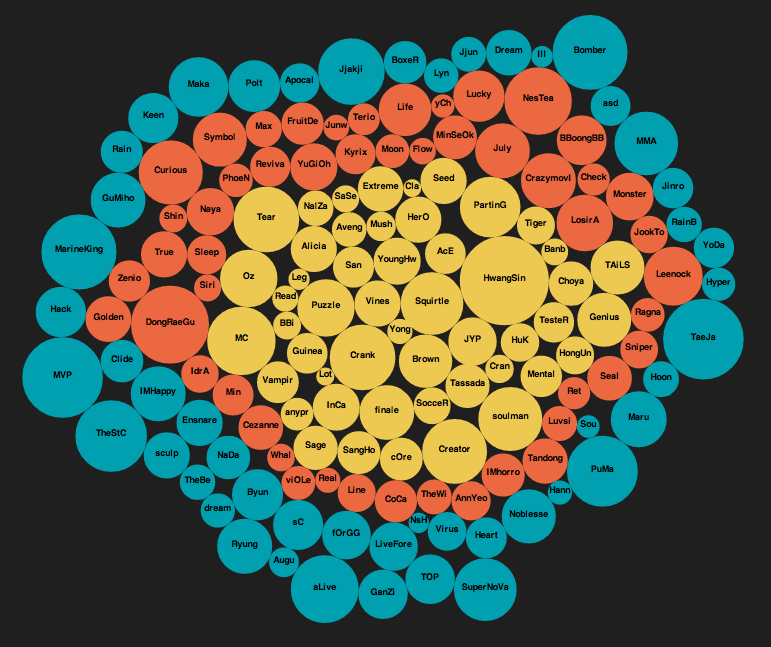
\includegraphics[scale=.35]{pics/bubble_players.png}
  \caption{High-Performing Players - Zerg is Red, Terran is Blue, Protoss is Yellow.  Larger is better.}
\end{figure}
\begin{figure}[t]
  \centering
  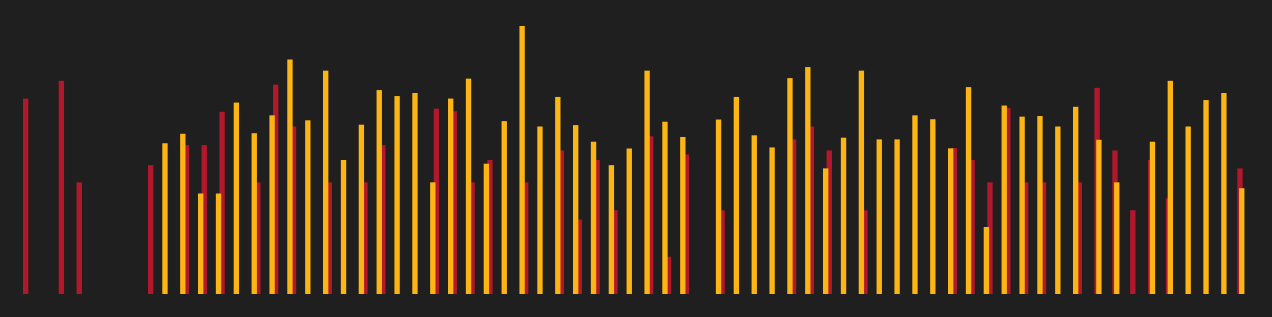
\includegraphics[scale=.25]{pics/bars_zvp.png}
  \caption{Protoss vs. Zerg win rates over time; Yellow is Protoss, Red is Zerg}
\end{figure}

\subsection{Finding High-Performing Players}
Finding high-performing players was a difficult task.  Initially, the approach of simply comparing player win rates was attempted, but was a miserable failure.  One critical feature of this datset was that there are a large number of distinct players, and most of them have only played a few matches (specifically, these are players that played in one or two tournaments, and stopped playing afterwards).  Thus, comparing win rates for players that have played 2-5 matches is clearly unfair to players who have played hundreds of matches.\\
In professional StarCraft, playing more matches is also indicative of skill.  In order to get invited to more tournaments, players must perform well in previous tournaments or risk being dropped from the professional scene altogether.  Therefore, one key observation was that the number of games played is a significant indicator for player skill.\\
Thus, we settled on using a standard rating for a binomial proportion, known as the lower bound of the Wilson score:
\[
\frac{{ {\hat p + \frac{{1}}{{2n}}
 z_{1- \alpha / 2}^2  \pm z_{1- \alpha / 2}
\sqrt {\frac{{\hat p\left( {1 - \hat p} \right)}}{n} + \frac{{z_{1- \alpha / 2}^2}}
{{4n^2}} }} }}
{{ {1 + \frac{{1}}{n}} z_{1- \alpha / 2}^2 }}
\]\\
This ended up as a very strong indicator for strong players - players regarded as the best StarCraft players also had a very high skill confidence.  We also found players who were not as highly regarded amongst the high ratings - one Protoss player was found to have many games played and a ~60\% win rate, and wasn't noticed by the public.  This was due to his relatively low exposure by the media, although he was performing at a top-tier level.

\subsection{Race Balance in the Professional Scene}
Another idea we wanted to visualize was racial balance in the professional scene.  Each race plays differently and one race may be vastly favored in a particular matchup.  In this visualization, we wanted to find if racial imbalances really existed in the professional Starcraft scene.  To do this, we took win percentages for each race, and compared them over time.\\

We can see that Protoss win rates are significantly higher than Zerg win rates for at least half the time period shown in the chart.  Until about 60\% of the way through, Protoss players have consistently had higher win rates than Zerg players.  However, after a little more than halfway through, Zerg win rates begin significantly increasing (and frequently outperforming Protoss win rates).  This point is actually in mid-September 2011, when a balance patch was released for StarCraft increasing the effectiveness of Zerg units.  This shifted the professional metagame for awhile, reducing Protoss win rates significantly.
